
% ---------------------------- comment out when compiling the full document -------------------
\documentclass[11pt]{mytustyle}  % default square logo 
\usepackage{amssymb}
\usepackage{caption}
\usepackage{upgreek}
\usepackage{subfig}
\begin{document}
\baselineskip=16pt
% ---------------------------------------------------------------------------------------------------------------


% ---------------------------------------------------------------------------------------------------------------
\chapter{Experimental results}
% ---------------------------------------------------------------------------------------------------------------
This chapter contains the measurement results of data taken with diamond sensors. The description of measurement setup (section~\ref{sec:meassetup}) and the experimental technique (section~\ref{sec:exptech}) is followed by discussion of limitations in sections \ref{sec:noiselimit}, \ref{sec:templimit} and \ref{sec:radlimit}.

The aim of this chapter is to compare the experimentally acquired data with the theory from the previous chapter. 

% ---------------------------------------------------------------------------------------------------------------
\section{Measurement setup}
% ---------------------------------------------------------------------------------------------------------------
\label{sec:meassetup}

The measurement chain consists of three main parts: a diamond sensor, a signal preamplifier and a readout device, as seen in diagram~\ref{fig:ro-chain}. 

The signals propagating along the analogue chain are fast and with low amplitudes, which gives rise to importance of RF shielding. For instance, the sensor carrier has to be RF-tight to shield from external interferences. Also, the connection between the carrier and the preamplifier has to be as short as possible to avoid capacitive signal losses in the transmission line. Finally, the system needs to be grounded properly.

\begin{figure}
\centering
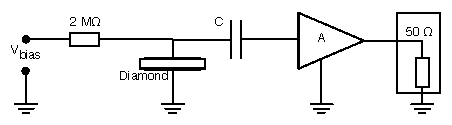
\includegraphics[width=0.8\textwidth]{plots/ro-chain}
\caption{Diagram of a diamond detector readout chain.}
\label{fig:ro-chain}
\end{figure}


\subsection{Preamplifiers}
\label{sec:preamps}
Two preamplifiers were used for the measurements, both embedded in an RF-tight aluminium box to reduce the noise pickup. Both have an AC coupled input and a 50~$\Upomega$ output.

\emph{CIVIDEC C2} is a fast current preamplifier with a 2~GHz bandwidth limit. It is used for TCT measurements because if its fast response and a good SNR.

\emph{CIVIDEC Cx} is a charge shaping amplifier. Its high SNR (low noise of 400~electrons and gain of 8.2~mV/fC) makes it a good choice for spectroscopic measurements with diamond sensors.

\begin{figure}[!ht]
%\centering
\begin{tabular}{cccc}
\subfloat[Cx charge shaping preamplifier]{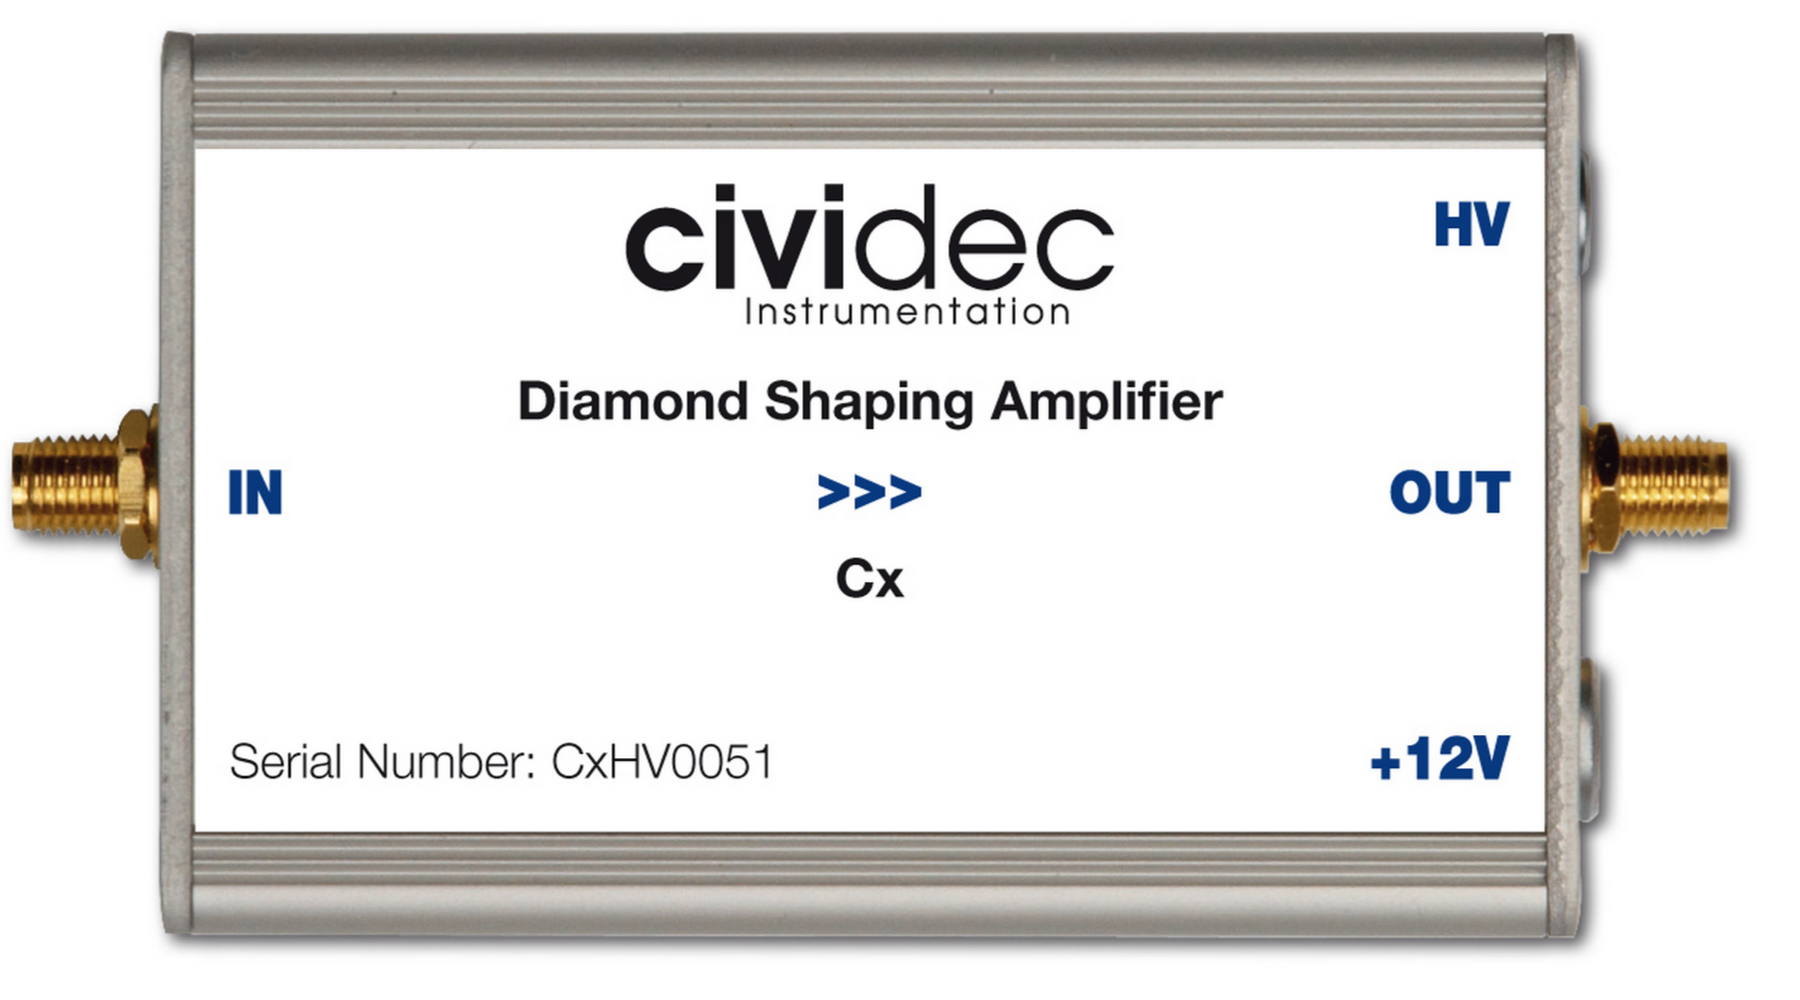
\includegraphics[width=0.45\textwidth]{pics/Cx} \label{fig:ampcx}} &
\subfloat[C2 fast charge preamplifier]{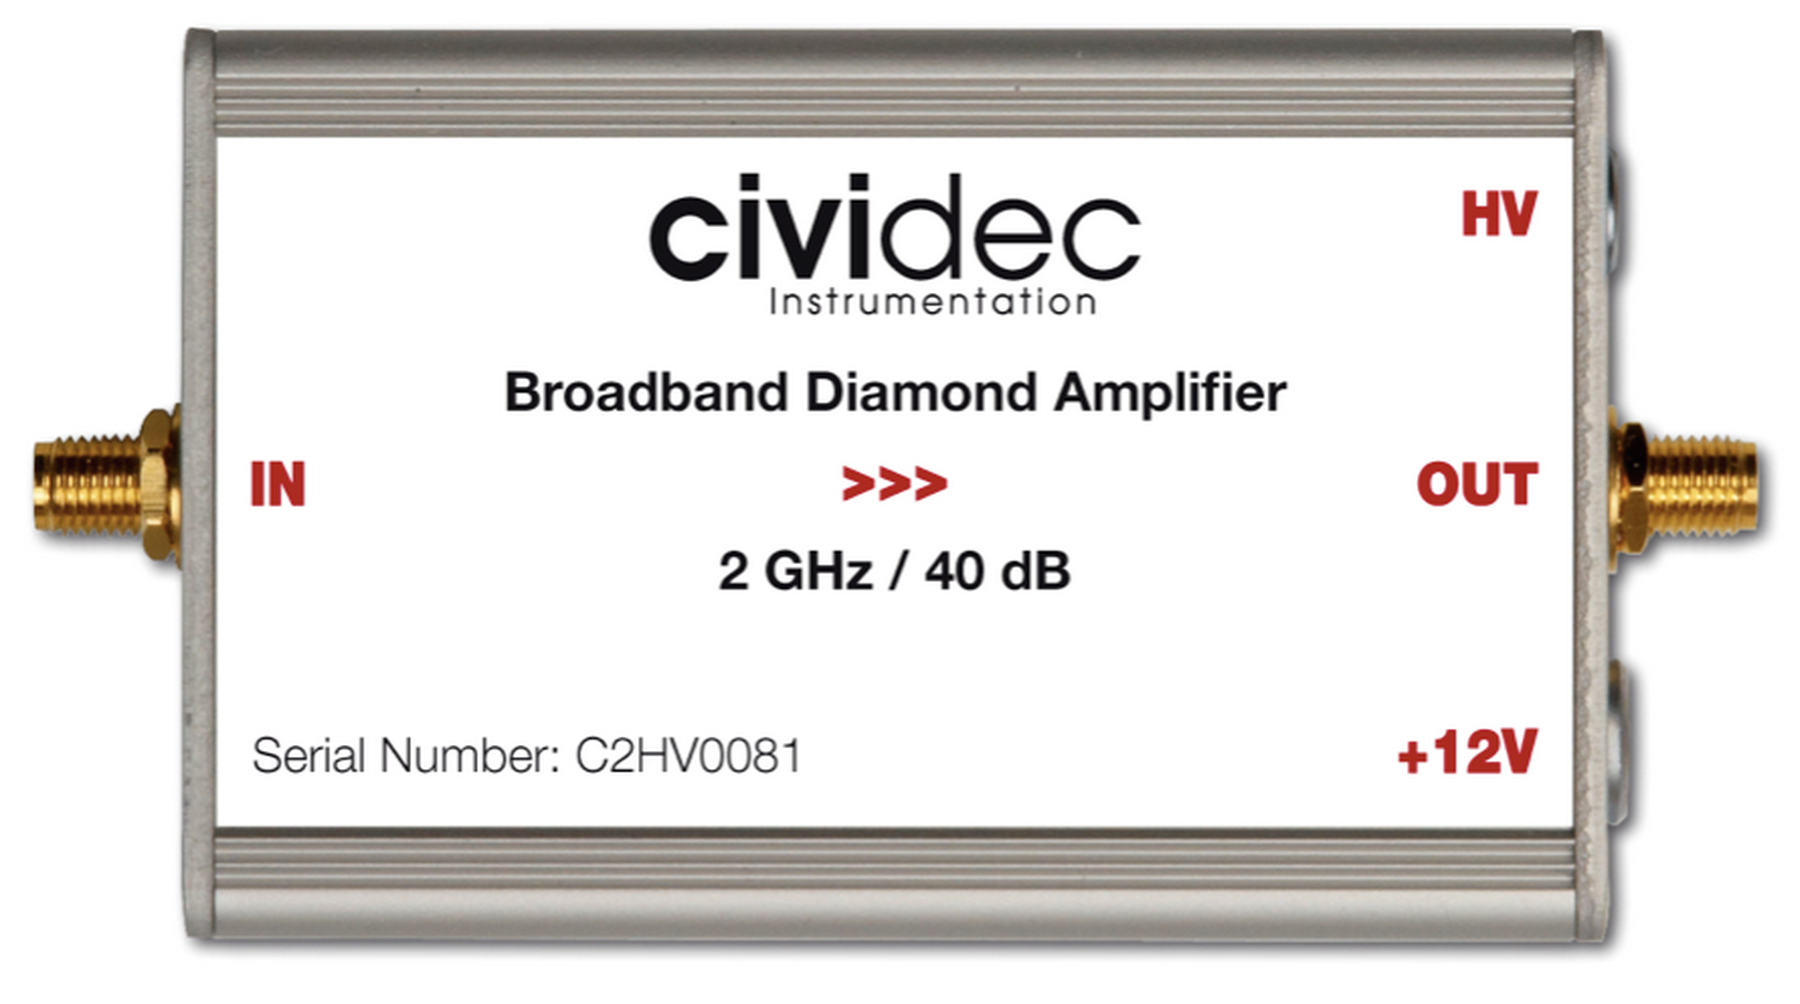
\includegraphics[width=0.45\textwidth]{pics/C2}  \label{fig:ampc2}}
\end{tabular}
\caption{Thermal neutron measurement setup}
\end{figure}


\subsubsection{Diamond samples}
\label{sec:diamsam}

\subsubsection{Readout device}
\label{sec:readoutdev}
Oscilloscopes are the most versatile analogue signal readout devices - fast to set up and reliable. It is important, though, to choose an oscilloscope with high enough bandwidth, especially for the fast current preamplifier signals. The choice for this setup was a 1~GHz and a 2~GHz option from the LeCroy WaveRunner family.

\subsection{Cryogenic setup}
\label{sec:cryosetup}








% ---------------------------------------------------------------------------------------------------------------
\section{Experimental technique}
% ---------------------------------------------------------------------------------------------------------------
\label{sec:exptech}





Noise limitations

Lab measurements

Temperature and radiation limitations

Transient current technique

Charge - before and after irradiation

compare with RD42 results

Generation of trapping centres, reference KIT, Marok, Harris�

IIa

%\section{Pulse formation}
\section{Noise limitations}
\label{sec:noiselimit}
TO DO: Take 8 runs with the 2GHz oscilloscope while increasing the noise. 

\section{Temperature limitations}
\label{sec:templimit}


\section{Radiation limitations}
\label{sec:radlimit}
Exposure to ionising radiation degrades sensors. 


\section{Conclusion}
\label{sec:radlimit}



% ---------------------------- comment out when compiling the full document -------------------
\end{document}
% ---------------------------------------------------------------------------------------------------------------


